\subsection{The Room class}
\label{subsec:application:building_the_model:the_room_class}

The second step is very similar to the previous step, as yet another type will be introduced. This time around, the class type for rooms is introduced. \cref{subsec:library_of_transformations:type_level_transformations:regular_classes} is used to introduce the class type, while on the instance level, \cref{subsec:library_of_transformations:instance_level_transformations:plain_objects} is used to introduce the house objects.

The $name$ of the new room type is $.\type{Room}$. However, this time, no objects of the room type will be introduced just yet, therefore, $objects = \{\}$. Moreover, there is no need to define $fid$. The following model is obtained:

\LTXtable{\textwidth}{tex/06_application/02_building_the_model/tables/02_the_room_class.tex}

\begin{figure}[p]
    \centering
    \begin{subfigure}{0.98\textwidth}
        \centering
        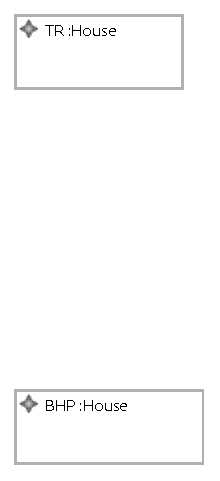
\includegraphics{images/06_application/instance_model/step02.pdf}
        \caption{Instance Model $Im_2$}
        \label{fig:application:building_the_model:the_room_class:ecore:instance_model}
    \end{subfigure}
    \\
    \begin{subfigure}{0.98\textwidth}
        \centering
        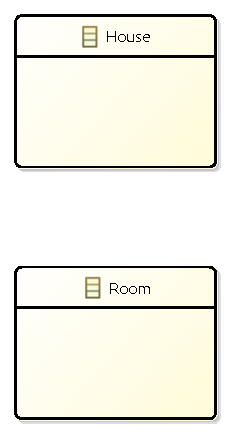
\includegraphics{images/06_application/type_model/step02.pdf}
        \caption{Type Model $Tm_2$}
        \label{fig:application:building_the_model:the_room_class:ecore:type_model}
    \end{subfigure}
    \caption{The Ecore model after step 2}
    \label{fig:application:building_the_model:the_room_class:ecore}
\end{figure}

\begin{figure}[p]
    \centering
    \begin{subfigure}{0.98\textwidth}
        \centering
        % To use this figure in your LaTeX document
% import the package groove/resources/groove2tikz.sty
%
\begin{tikzpicture}[scale=\tikzscale,name prefix=step02-]
\node[basic_node] (n0) at (2.680, -1.040) {\ml{\uline{\textit{BHP}} : \textbf{House}}};
\node[basic_node] (n1) at (2.660, -0.340) {\ml{\uline{\textit{TR}} : \textbf{House}}};

\end{tikzpicture}

        \caption{Instance Graph $IG_2$}
        \label{fig:application:building_the_model:the_room_class:groove:instance_graph}
    \end{subfigure}
    \\
    \begin{subfigure}{0.98\textwidth}
        \centering
        % To use this figure in your LaTeX document
% import the package groove/resources/groove2tikz.sty
%
\begin{tikzpicture}[scale=\tikzscale,name prefix=step02-]
\node[basic_node] (n0) at (2.680, -1.040) {\ml{\uline{\textit{BHP}} : \textbf{House}}};
\node[basic_node] (n1) at (2.660, -0.340) {\ml{\uline{\textit{TR}} : \textbf{House}}};

\end{tikzpicture}

        \caption{Type Graph $TG_2$}
        \label{fig:application:building_the_model:the_room_class:groove:type_graph}
    \end{subfigure}
    \caption{The GROOVE graphs after step 2}
    \label{fig:application:building_the_model:the_room_class:groove}
\end{figure}

A visual representation of $Tm_2$ and $Im_2$ can be found in \cref{fig:application:building_the_model:the_room_class:ecore}. Similarly, a visual representation of $TG_2$ and $IG_2$ can be found in \cref{fig:application:building_the_model:the_room_class:groove}. Please note that because of the definitions of $f_2(Im_2)$ and $f'_2(IG_2)$, we have that $f_2(Im_2) = IG_2$ and $f'_2(IG_2) = Im_2$. Furthermore, $f_2(Im_2)$ and $f'_2(IG_2)$ are valid mapping functions themselves, such that they can be combined with another mapping function in the next step.

The visual representation of the models is still not stunning, mainly because the instance model and instance graph have not changed during this step. These are unchanged because the room objects will all be contained by houses, and therefore need to be introduced later to keep the model and graphs valid.

\afterpage{\FloatBarrier}